\section{Tests on the MeerKAT LMC observation}\label{results}
For algorithmic testing


	
\begin{figure}[h]
	\centering
	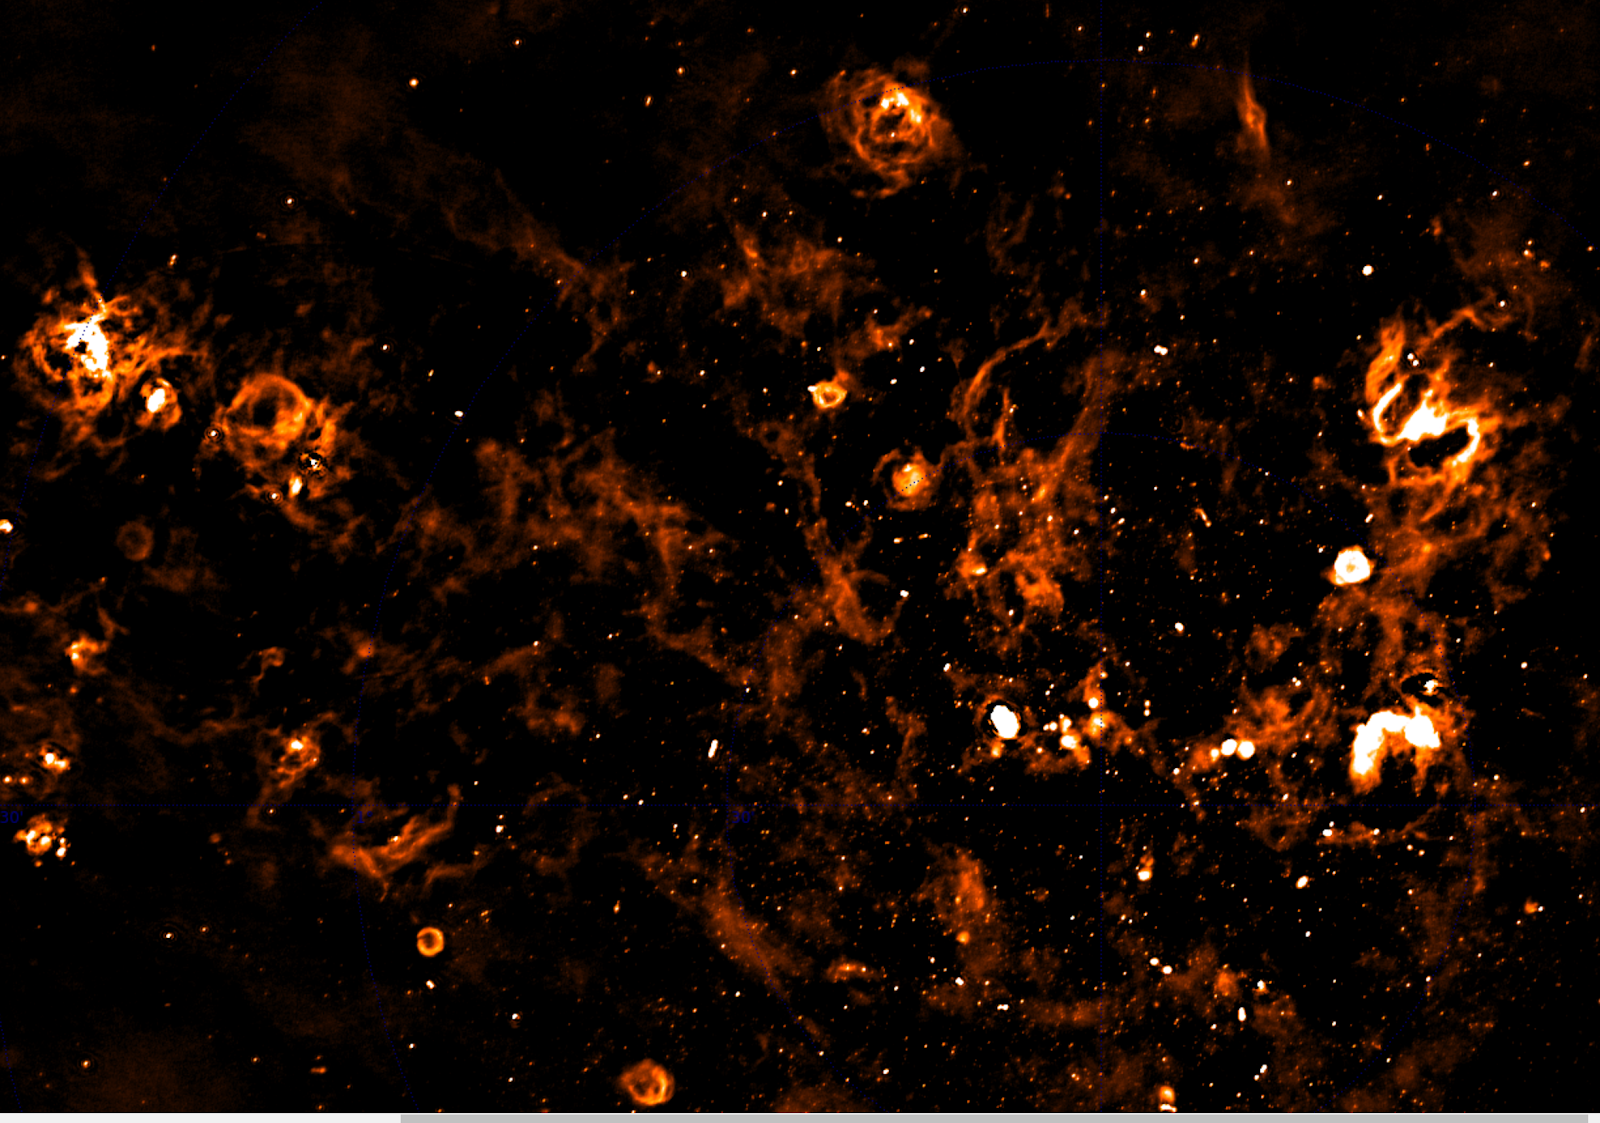
\includegraphics[width=0.80\linewidth]{./chapters/10.results/LMC/meerkat.png}
	\caption{Radio interferometer system}
	\label{results:radio}
\end{figure}



\subsection{Comparison with CLEAN reconstruction}

\subsection{Speedup}

\subsection{PSF as the limiting factor}


\subsection{Approximation of gradients}

\subsubsection{Major Cycle convergence}
Putting it all together

We have the Minor Cycle, which is easy to converge.

Coordinate Descent Path optimization \cite{friedman2010regularization}
Danger that CD takes too many pixel into a Major Cycle. Lower bound per iteration, PSF sidelobe
can still be too low, danger when many psf sidelobes overlap


We are in the realm of convolution. Remember that a convolution in image space is a multiplication in fourier space.
We can multiply

\subsection{Wall clock time}
\begin{figure}[h]
	\centering
	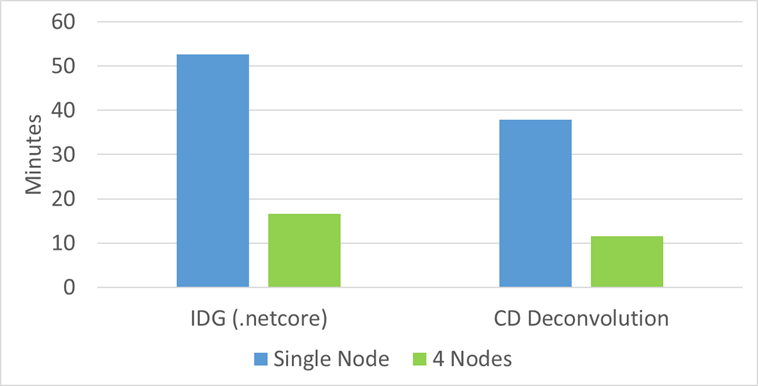
\includegraphics[width=0.80\linewidth]{./chapters/10.results/wall-clock-time.png}
	\caption{Wall-clock time of the distributed reconstruction}
	\label{results:time:fig}
\end{figure}
